\section{Readout Electronics}
\label{sec:dp-pds-electronics}

%%%%%%%%%%%%%%%%%%%%%%%%%%%%%%%%%
\subsection{Photomultiplier High Voltage Dividers}
\label{sec:fddp-pd-4.1}

The \dword{pmt} has a grounded cathode and a positive \dword{hv} applied to the anode. A single cable for each \dword{pmt} carries both power and signal. This configuration, which requires half as many cables and feedthroughs on the detector compared to the negative voltage configuration, offers a clear advantage given the large number of \dwords{pmt} in the detector. In addition, the cathode grounding shows fewer dark counts than the anode grounding scheme. Although a coupling capacitor must be used to separate the \dword{hv} from the \dword{pmt} signal, this signal and power splitting can be done externally, mitigating this drawback.  Figure~\ref{fig:dppd_4_1} shows the positive power supply and cathode grounding scheme.

\begin{dunefigure}[Positive power supply and cathode grounding scheme.]{fig:dppd_4_1}
{Positive power supply and cathode grounding scheme.}
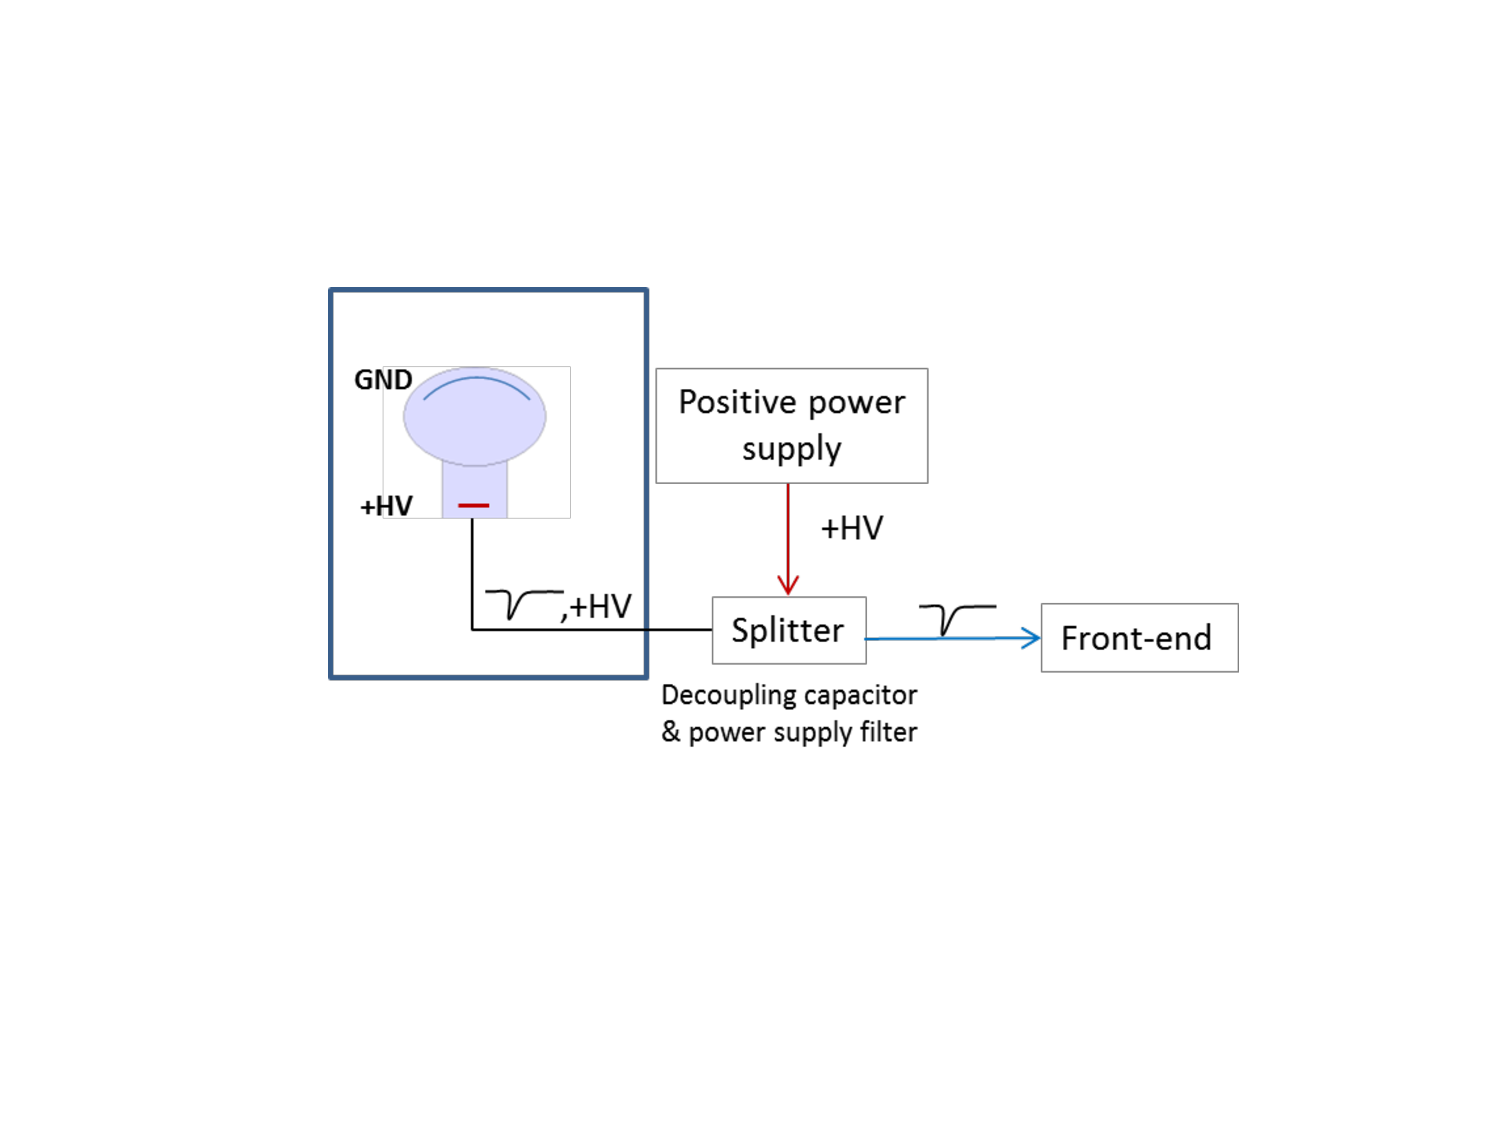
\includegraphics[width=0.6\textwidth]{dppd_4_1}
\end{dunefigure}

The \dword{pmt} base circuit uses only resistors and capacitors. The components are carefully selected and tested to minimize the variations in their characteristics with temperature. The polarization current of the voltage divider (total circuit resistance) is chosen to fit the \dword{pmt} light linearity range (up to \SI{200}{PEs}) and maximum power (\SI{<0.2}{W/\dword{pmt}}) requirements. The dynodes' voltage ratio will follow the manufacturer recommendations for increasing linearity range on the space-charge effect area (tapered divider). In addition, capacitors are added to the last stages in order to increase the \dword{pmt} linearity in pulsed mode.

The connection between the \dword{pmt} base and the \fdth is done by the RG-303/U cable, being selected for its low attenuation and its proven reliability in cryogenic environments. The short cable is directly soldered to the \dword{pmt} base on one side, and it ends with an SHV connector on the other side for attachment to the long \dword{hv} cable. The long cable connects to the feedthrough flange.

%This cable is directly soldered to the \dword{pmt} base on one side, and it ends with an SHV connector on the other side for attachment to the long \dword{hv} cables coming from the feedthrough flanges. 

%%%%%%%%%%%%%%%%%%%%%%%%%%%%%%%%%
\subsection{High Voltage and Signal Splitters}
\label{sec:fddp-pd-4.2}

\Dword{hv} and signal splitters 
are used to separate the fast \dword{pmt} response signal from the positive \dword{hv} with capacitive decoupling. 
A low-pass filter between the \dword{hv} supply and the \dword{pmt} reduces the noise.

It is possible for radiated electromagnetic interference (EMI) to be picked up by the cables, and conducted noise from the \dword{hv} power supply to be synchronous across many \dword{pmt} channels (i.e., coherent noise). This noise could add up to produce false detector triggers. Since the \dword{pmt} signal can be as low as a few \si{mV},
control of the EMI over the circuit is very important. The splitter \dword{hv} input filter is intended to reduce the EMI induced and conducted by the power supply cables. Enclosing each splitter channel in its own metallic grounded box reduces the EMI directly received in the splitter circuit and 
the cross-talk between different splitter channels.

Figure \ref{fig:dppd_4_2} shows a generic splitter circuit where R1 and C1 form the \dword{hv} input low-pass filter (with a cut-off frequency below \SI{60}{Hz}). The resistor R7 and the  \dword{led} are for safety purposes only, warning when \dword{hv} is applied to the splitter. The C4 capacitor splits the signal coming from the \dword{pmt} from the \dword{hv}, and R2 prevents the \dword{pmt} signal from going to ground through the C1 capacitor. R4 and R5 are \SI{0}{\ohm} optional resistors that allow some flexibility in the grounding configuration. Finally, R3 ensures the discharging of C4 if the splitter is not connected to the \SI{50}{\ohm} input at the \dword{daq} system. The RC constant of the capacitor C4 and the load (\SI{50}{\ohm}) must be as large as possible to minimize baseline oscillations due to the charge-discharge of the capacitor. Values of C4 between \SI{150}{nF} and \SI{300}{nF} have already been tested. Figure \ref{fig:dppd_4_3} shows a picture of the \dword{hv}/signal splitter box of \dword{pddp}.

\begin{dunefigure}[Generic splitter circuit diagram.]{fig:dppd_4_2}
{Generic splitter circuit diagram.}
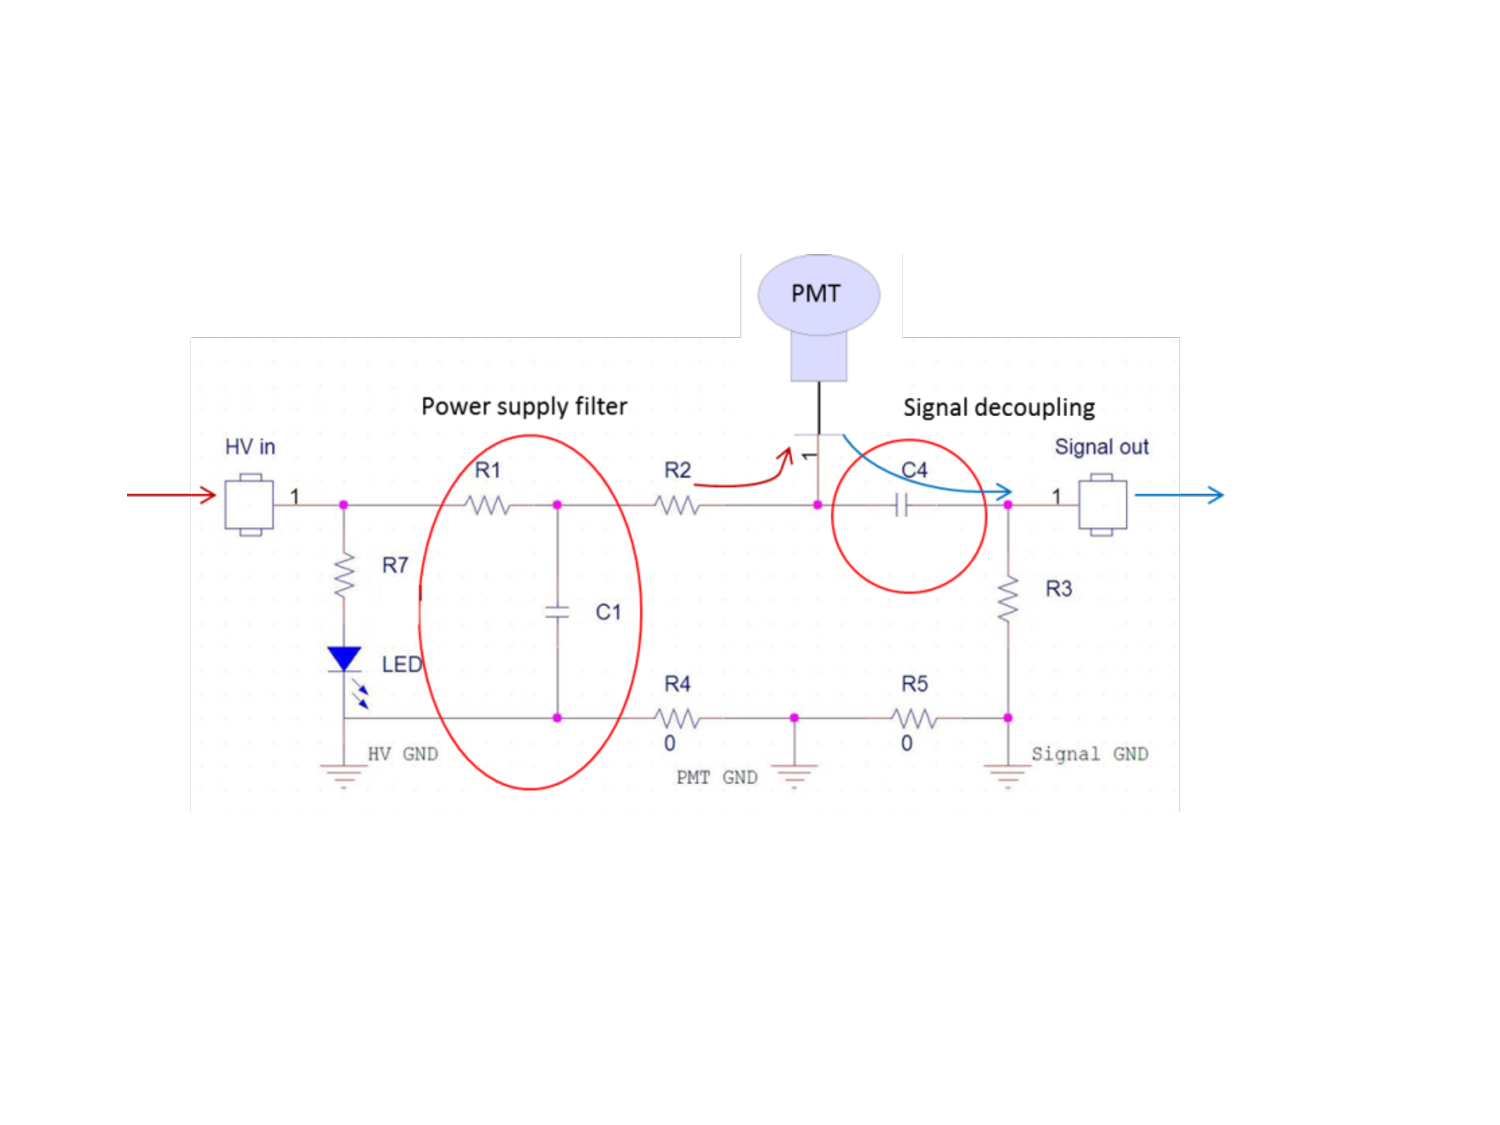
\includegraphics[width=0.85\textwidth]{dppd_4_2}
\end{dunefigure}

\begin{dunefigure}[Picture of the splitter box for \dword{pddp}.]{fig:dppd_4_3}
{Picture of the splitter box for \dword{pddp}.}
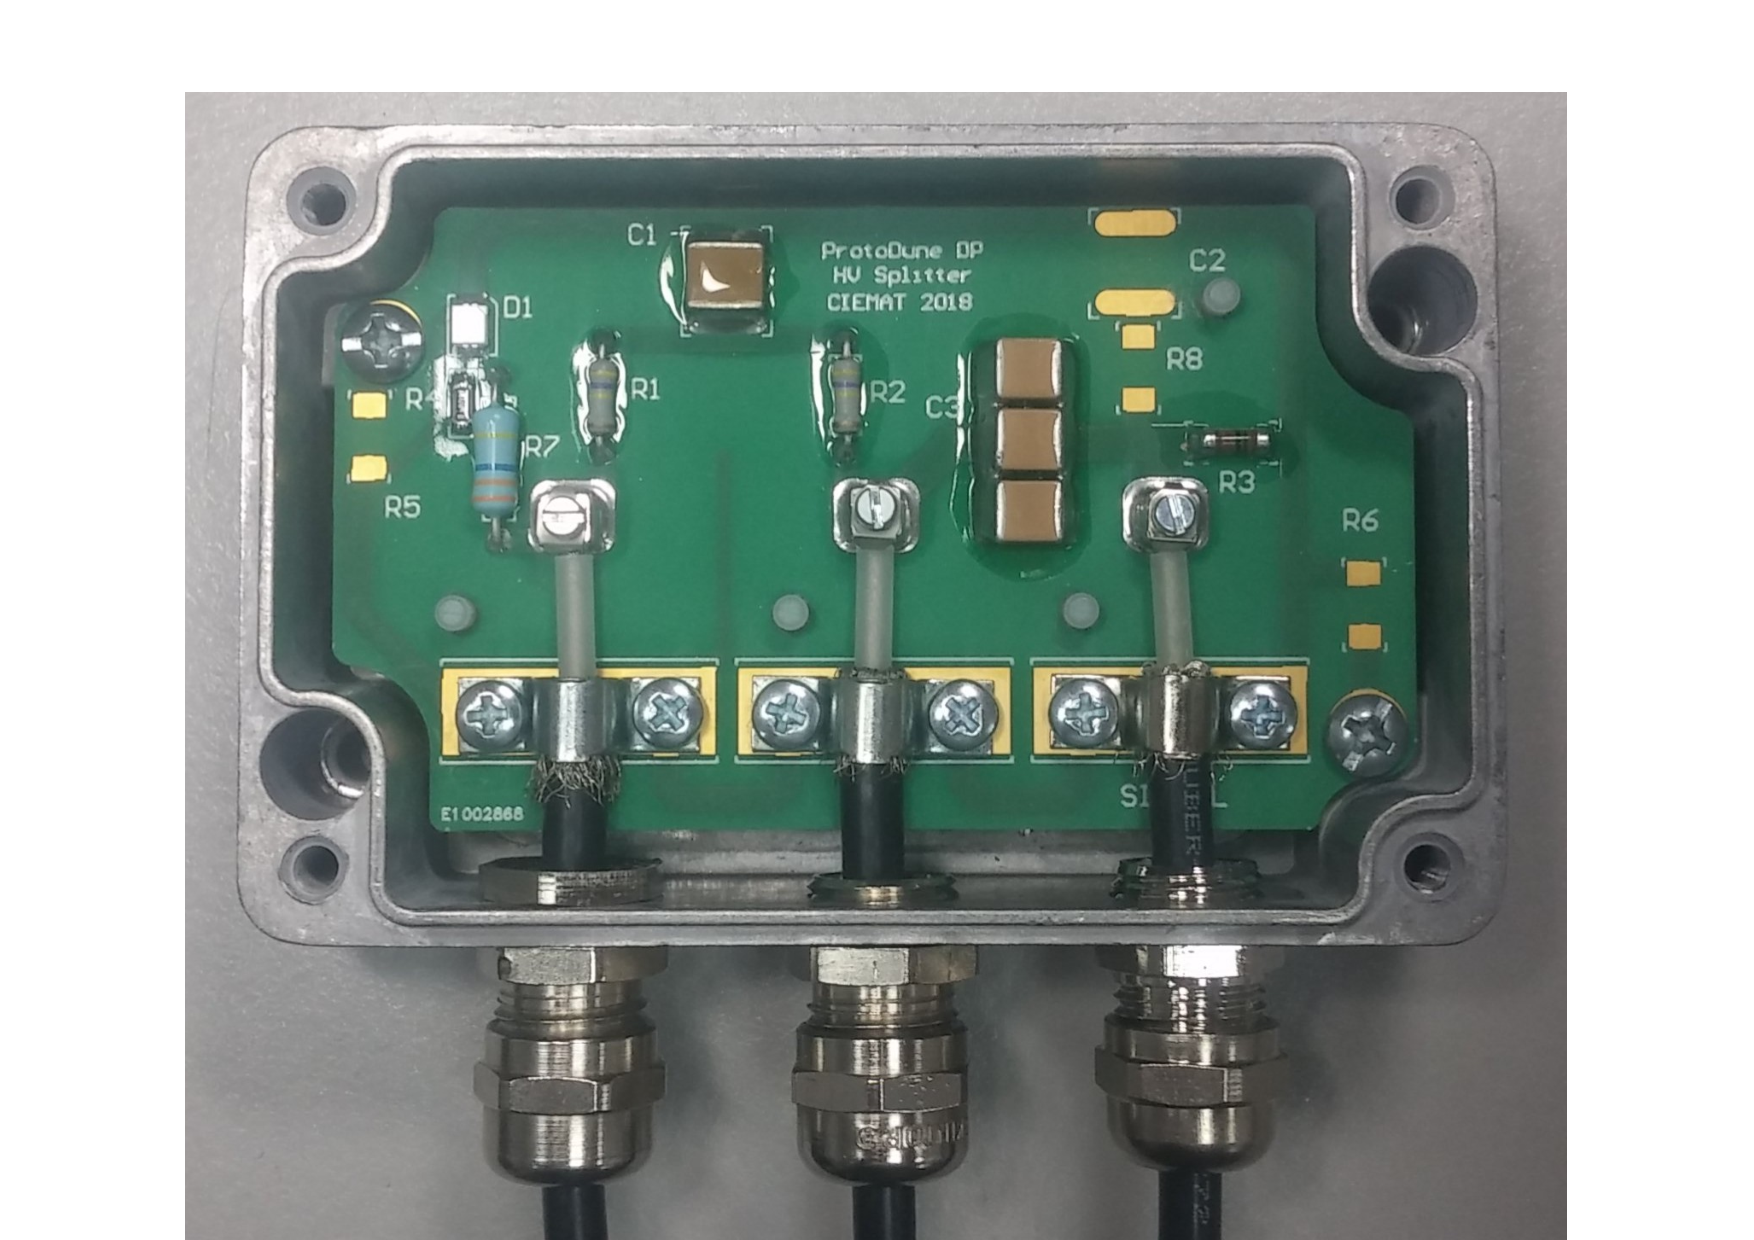
\includegraphics[width=0.5\textwidth]{dppd_4_n3}
\end{dunefigure}

For the connections between the \dword{hv} power supply and the splitters, and between the splitters and the cryostat \fdth{}s, the HTC 50-3-2 cables have been chosen as baseline. The HTC 50-3-2 has a similar attenuation as the RG-303/U (used inside the cryostat), but with a factor of \numrange{8}{10} lower cost. Both cables are attached on one side directly to the \dword{hv} splitter and have an SHV connector on the other end. An RG-58 cable terminated on the connector required by the light readout card provides the connection between the splitter and the card. The \dword{pmt} readout card is described in Chapter~\ref{ch:dp-tpcelec}.

%\fixme{Add Antonio's picture of \dword{pddp} HV/signal splitter.}

%%%%%%%%%%%%%%%%%%%%%%%%%%%%%%%%%
%\subsection{Signal Readout Requirements}
\subsection{Signal Readout}
\label{sec:fddp-pd-4.3}

In order to meet the physics requirements, the information that needs to be extracted from the \dword{pmt} signals is the following:

\begin{itemize}
\item S1 fast component shape, charge and timing.
\item S1 slow component shape.
\item S2 shape, charge and timing (distance from S1 and duration).
\item Single \phel (SPE) charge spectrum for gain calculation during \dword{pmt} calibration.
\item Trigger signal generation by the coincidence of several \dword{pmt} signals.
\end{itemize}

%%At this moment, we do not have an estimate of the \textbf{dynamic range }of the light that could reach the \dwords{pmt} on the \dword{dpmod}. Our calculations are based on the signals detected by the \dwords{pmt} on the  \dword{wa105} $3\times1\times1$\,m$^3$ detector. Although this prototype has a different dimension from the \dword{dpmod}, it is the only reference that we have for these estimates, until the \dword{pddp} detector and simulations are operational.
%There is currently no estimate on the dynamic range of the light expected to reach the \dwords{pmt} in the \dword{dpmod}. Our calculations are based on the signals detected by the \dwords{pmt} in the \dword{wa105}, % $3\times1\times1$\,m$^3$ detector. Although this prototype has a 
%which has quite different dimensions from the \dword{dpmod}. However, it is the only available reference %that we have for these estimates, until the \dword{pddp} and simulations are operational.

In general, the \dword{pmt} signal dynamic range goes from the \si{mV} level to several volts (over \SI{50}{\ohm} load). The lower limit of the PMT dynamic range is given by the lowest level of the SPE signal that meets the signal to noise ratio specification. So, the \dword{pmt} gain should be set at the value that makes the SPE level meet this condition. The upper limit of the dynamic range is given by the \dword{pmt} signal amplitude for the maximum number of PEs expected per sampling time unit. This amplitude can be calculated approximately as number of PEs $\times$ SPE amplitude (at the gain required to meet the S/N ratio at SPE level). Figure~\ref{fig:dppd_4_3_ab} shows the SPE waveforms (left) and amplitudes from the WA105 at different voltages (right).
%During the operation of the \dword{wa105}, \dword{pmt} signals larger than \SI{2}{V} were observed with \dword{pmt} gains around \num{e6}. %\num{10}$^6$. 
%Figure~\ref{fig:dppd_4_3_ab} shows the SPE waveforms (left) and amplitudes (right) for the \dword{wa105} at different voltages. The light levels in the \dword{dpmod} will have a larger dynamic range due to its large volume, therefore higher gains are required to see the far light signals. However, higher gains increase the output from closer light signals, requiring that the \dword{fe} electronics cover a large range of input voltages.To cover a dynamic range of \SI{10}{V} with a resolution below the \si{mV} level, \num{14} bits are necessary (least significant bit (LSB) $\sim$\SI{0.6}{mV}). For a dynamic range of \SI{2}{V}, \num{12} bits would be enough (LSB $\sim$\SI{0.5}{mV}).
%Results from \dword{pddp} and relevant simulations are needed to determine the required dynamic range.

\begin{dunefigure}[SPE waveforms and amplitudes from the WA105 at different voltages.]{fig:dppd_4_3_ab}{SPE waveforms (left) and amplitudes from the WA105 at different voltages (right).}
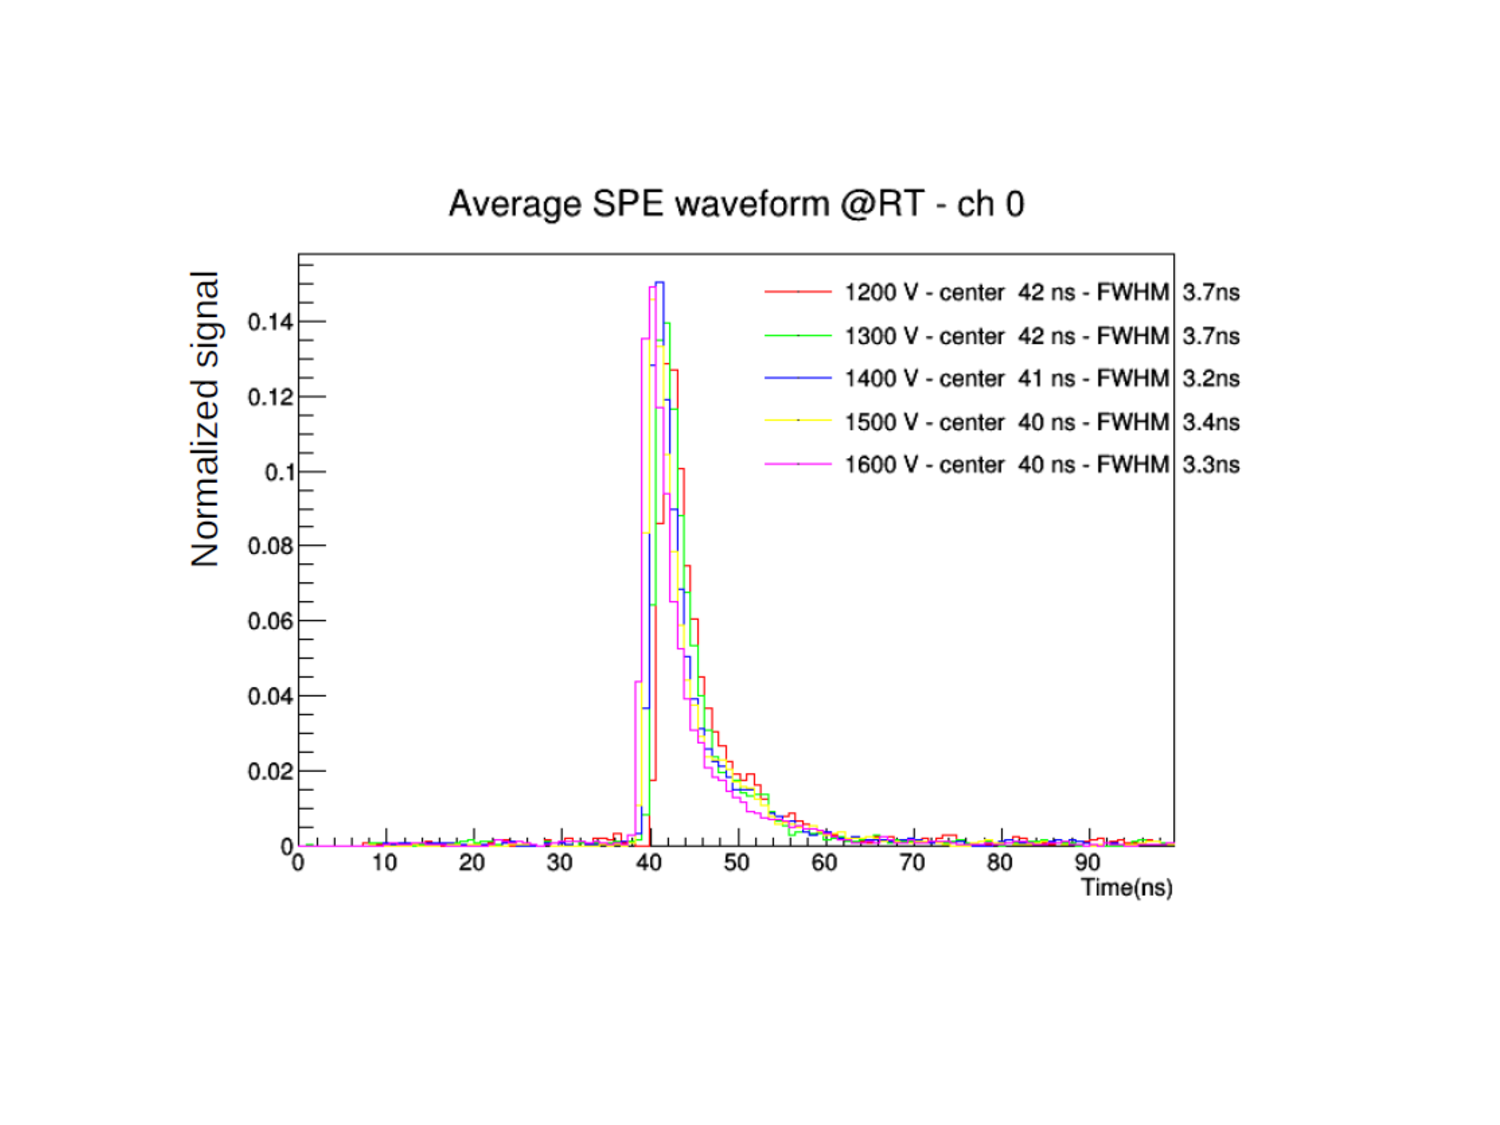
\includegraphics[width=0.47\textwidth]{dppd_4_3_a}
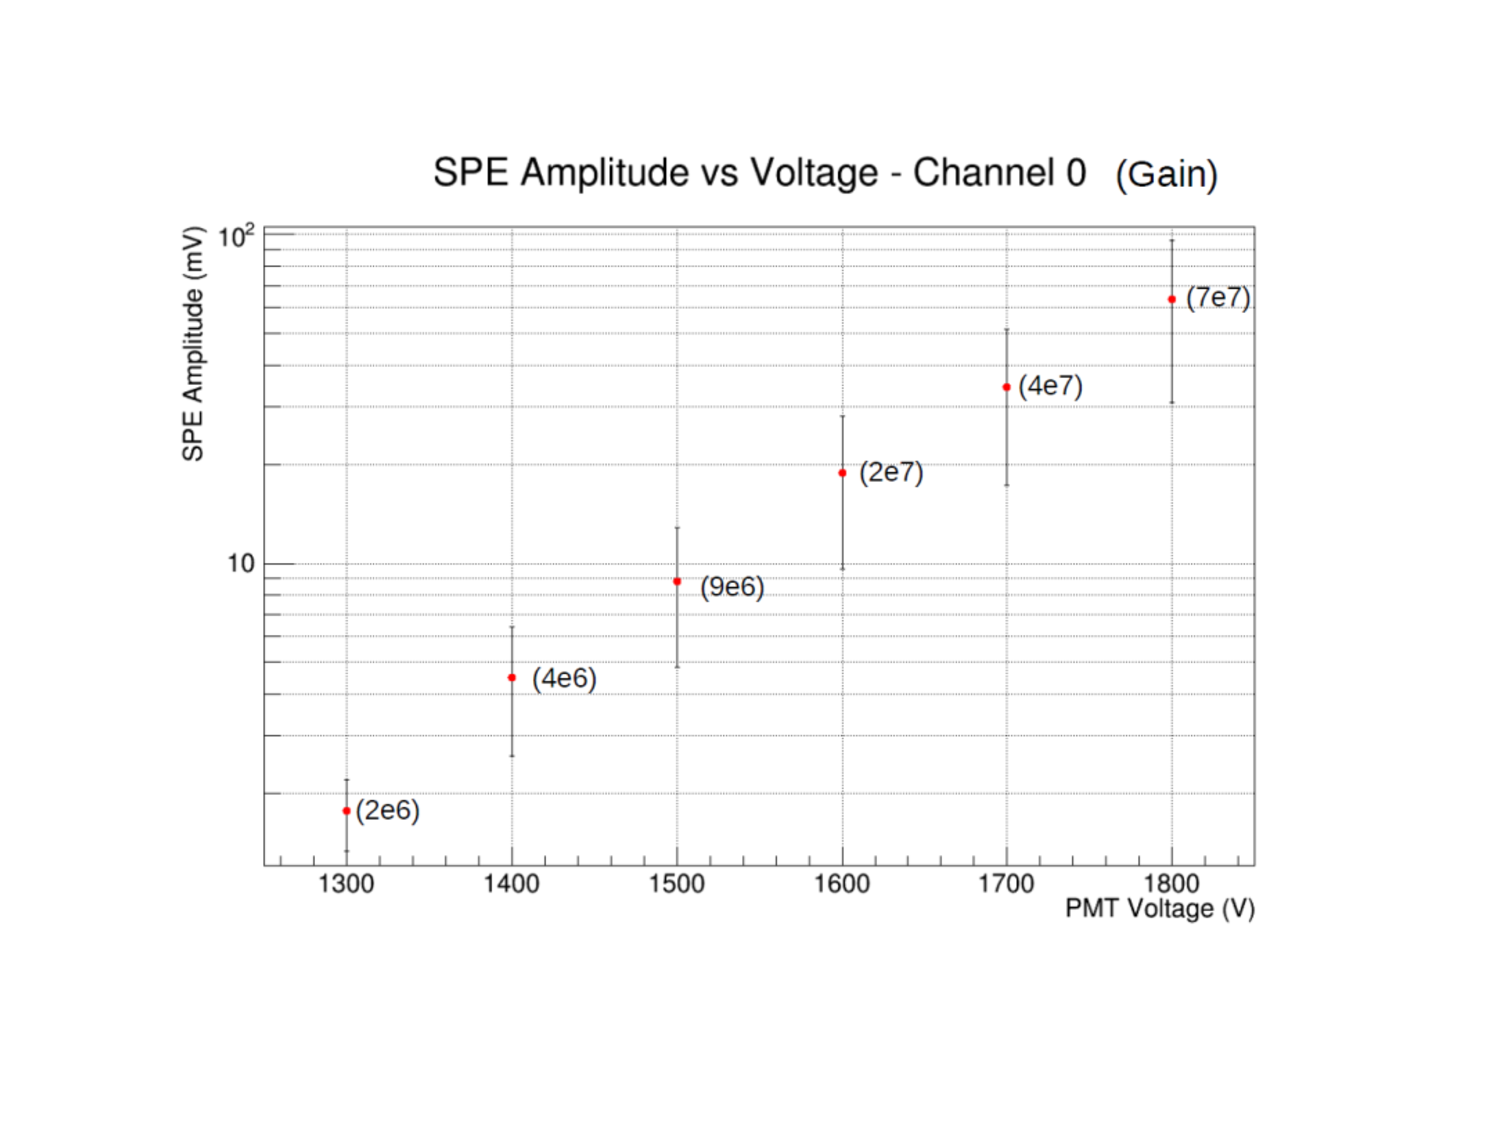
\includegraphics[width=0.47\textwidth]{dppd_4_3_b}
\end{dunefigure}

%In order to calculate the \dword{pmt} gains, the SPE charge measurement will be performed. Depending on the \dword{pmt} gain, the SPE amplitude varies from the \si{mV} level to hundreds of \si{mV}.%, as shown in Figure~\ref{fig:dppd_4_3_ab}. 
Due to the very long cables from the \dwords{pmt} to the \dword{fe} electronics, the noise into the cables could be high. If a noise level around \SI{1}{mV} is considered,  the \dword{pmt} gain must be set around \num{e7} to have the required S/N ratio of 5. The average SPE pulse width is around \SI{3.5}{ns} full width at half maximum (FWHM). If an accurate signal reconstruction is required, the sampling period should be of the level of the \si{\ns}. If only charge information is relevant, the sampling period can be higher but the signal must low-pass filtered before the sampling. This filtering has an impact on the signal level making the discrimination of the signal from the noise more difficult and requiring an increase of the \dword{pmt} gain to meet the S/N specification.

The sampling frequency also affects the time tagging precision. The time uncertainty due to the \dword{pmt} alone is around \SI{3}{ns} (transit time spread). Other factors, e.g., Rayleigh scattering, increase this uncertainty, as does the sampling period. Therefore, the higher the sampling frequency, the better for the detector performance at the cost of increased data rate and storage requirements.
%Results from \dword{pddp} and  simulations will help to determine the optimal sampling rate. In the  \dword{wa105} \SI{4}{ns} sampling was used to digitize waveforms.

%The rate of the events observed in the \dword{wa105} was around \SI{300}{kHz} with the threshold at the SPE level. The rate at the \dword{dpmod}, is not yet known, but expected to be much larger despite the underground location. The time-tagging system needs to process events at high rates to ensure that no events are lost. Figure~\ref{fig:dppd_4_3_c} shows the event rates for different trigger thresholds observed in the \dword{wa105}.

%\begin{dunefigure}[Event rates for different trigger thresholds observed in the \dword{wa105}.]{fig:dppd_4_3_c}{Event rates for different trigger thresholds observed in the \dword{wa105} .}
%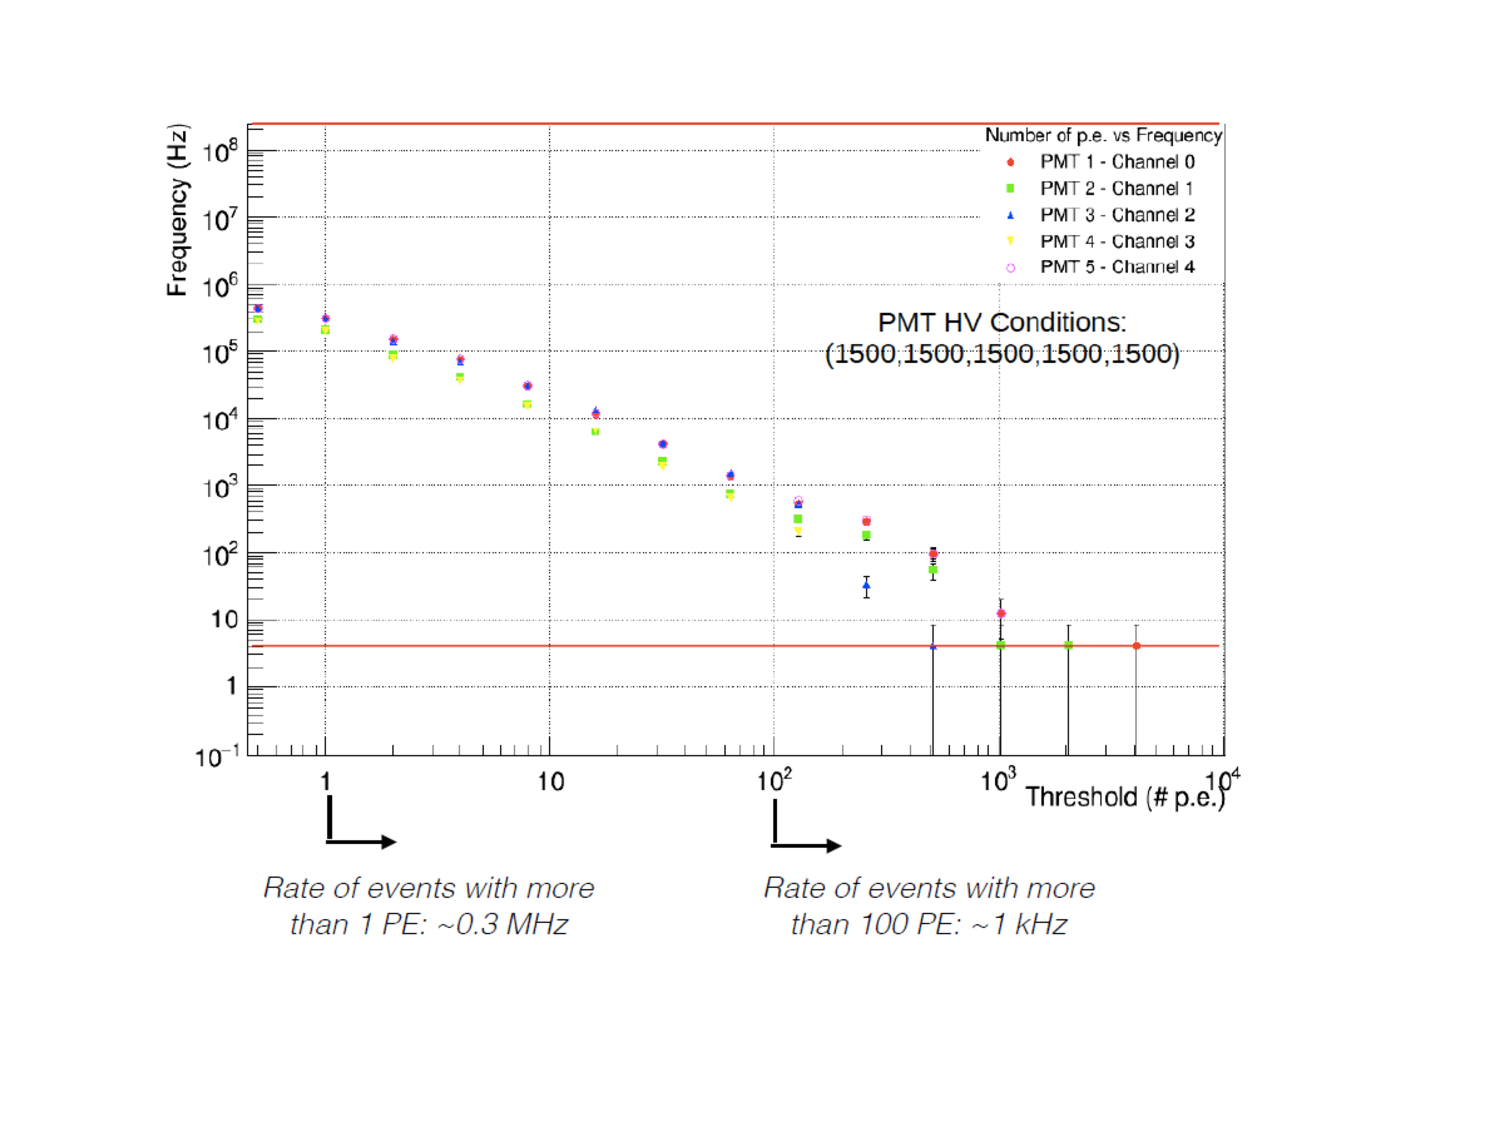
\includegraphics[width=0.6\textwidth]{dppd_4_3_c}
%\end{dunefigure}

The light signal has to be synchronized with the \dword{daq}. All the \dword{daq} electronics use the \dword{wr} protocol for synchronization. A dedicated \dword{wr} \dword{utca}~\cite{utca} slave node is on the light readout \dword{fe} electronics as sync receiver, distributing clocks to the different \dword{fe} cards.

Several \dword{pds} specifications that have an impact on the signal readout design, namely the required relative timing accuracy among hits, hit signal-to-noise ratio and analog range per channel, are listed in Table~\ref{tab:specs:just:DP-PDS}. 
